\documentclass[11pt]{article}
\usepackage[utf8]{inputenc}
\usepackage[T1]{fontenc}
\usepackage{amsmath,amssymb,amsfonts}
\usepackage{graphicx}
\usepackage{booktabs}
\usepackage{caption}
\usepackage{subcaption}
\usepackage{hyperref}
\usepackage{geometry}
\usepackage{xcolor}
\usepackage{natbib}
\usepackage{titlesec}

\geometry{margin=1in}
\graphicspath{{figures/}}
\hypersetup{
    colorlinks=true,
    linkcolor=blue,
    filecolor=magenta,
    urlcolor=cyan,
    pdftitle={A Decision-Support Framework for Subsurface Green Hydrogen Storage Site Selection: A Physics-Informed Multi-Objective Optimization Approach},
    pdfauthor={Kudakwashe Douglas Marara},
    pdfsubject={Hydrogen storage, site selection, physics-informed neural networks, geospatial optimization}
}

\title{A Decision-Support Framework for Subsurface Green Hydrogen Storage Site Selection:\\A Physics-Informed Multi-Objective Optimization Approach}

\author{
    Kudakwashe Douglas Marara\\
    University of Zimbabwe (BSc Hons Petroleum Chemistry, 2025)\\
    \texttt{kudakwashe.d.marara@gmail.com}
}

\date{}

\begin{document}

\maketitle

\begin{abstract}
The global energy transition requires large-scale, long-term hydrogen storage. Subsurface geological formations - depleted oil and gas fields and saline aquifers - offer the safest and most economical option. However, identifying optimal storage locations requires balancing competing factors: renewable energy potential, water availability, geological suitability, socio-economic constraints, and physics-based storage safety. No open-source decision-support framework currently integrates multi-objective geospatial optimization with physics-informed neural networks (PINNs) for hydrogen-brine interfacial tension (IFT) prediction. This paper presents a two-layer decision-support framework for subsurface green hydrogen storage site selection. The strategic screening layer performs regional suitability analysis using geospatial multi-objective optimization with weight sensitivity analysis and robustness mapping. The tactical planning layer integrates a PINN predicting H$_2$-brine IFT under reservoir conditions (pressure, temperature, salinity) with Peng-Robinson equation-of-state (PR-EOS) physics constraints, producing a spatially-varying safety penalty layer. Applied to a Southern Africa case study ($12^\circ$E--$22^\circ$E, $10^\circ$S--$20^\circ$S; Namibia, Botswana, western South Africa), the framework identifies 4.4\% of pixels as GO zones and 15.5\% as conditional GO, with candidate regions in the Etosha and Kalahari basins passing integrated go/no-go thresholds. The framework is open-source and transferable to other regions and energy-storage applications.

\textbf{Keywords:} hydrogen storage, site selection, multi-objective optimization, physics-informed neural networks, interfacial tension, geospatial decision support, Peng-Robinson equation of state
\end{abstract}

\section{Introduction}
\subsection{Decision Problem Framing}
The global hydrogen economy requires large-scale subsurface storage to balance seasonal renewable energy supply and demand. Geological formations - depleted oil and gas fields and saline aquifers - provide the safest and most cost-effective option for long-term, large-volume hydrogen storage. However, identifying the optimal storage location is a complex multi-criteria decision problem. It requires balancing renewable energy potential (for green hydrogen production), water availability (for electrolysis), geological suitability (basin type, caprock integrity, porosity), socio-economic factors (proximity to end-users, safety buffers from population centers), and physics-based storage safety constraints (H$_2$-brine interfacial tension and capillary trapping).

Decision-makers face deep uncertainty: no existing open-source tool integrates all these factors into a single, physics-informed geospatial framework. This gap is particularly acute in Africa and Europe, where hydrogen storage planning is nascent but critical for energy security and decarbonization goals.

\subsection{Novel Contribution}
This paper presents a two-layer decision-support framework for subsurface green hydrogen storage site selection:

\begin{enumerate}
    \item \textbf{Strategic screening layer} - a regional geospatial multi-objective optimization that ranks pixels by suitability across solar, water, and population layers, with weight sensitivity analysis and robustness mapping to identify sites stable under varying stakeholder preferences.
    \item \textbf{Tactical planning layer} - a site-specific analysis integrating a Physics-Informed Neural Network (PINN) for H$_2$-brine interfacial tension (IFT) prediction, constrained by the Peng-Robinson equation of state, producing a spatially-varying safety penalty layer that adjusts suitability scores for capillary trapping risk.
    \item \textbf{Decision-ready output} - integrated go/no-go recommendations with risk ranges, expressed as geospatial rasters suitable for direct use by planners, investors, and policymakers.
\end{enumerate}

The framework is demonstrated on a Southern Africa case study and is designed for transferability to other regions and energy-storage applications (e.g., carbon capture and storage, multi-component gas storage).

\section{Literature Review}
\subsection{Multi-Objective Decision Analysis for Energy Infrastructure}
Multi-criteria decision analysis (MCDA) and weighted overlay methods are well-established for energy infrastructure siting, including solar and wind farm location. However, applications specifically targeting subsurface hydrogen storage site selection remain limited. Existing approaches often use static, equal weights and lack systematic sensitivity analysis or robustness quantification under deep uncertainty.

\subsection{Geospatial Site Selection for Energy Infrastructure}
GIS-based weighted overlay and analytic hierarchy processes (AHP) are widely used for renewable energy siting. Few studies extend these methods to subsurface storage, where geological and petrophysical constraints dominate. Robustness mapping - identifying sites stable across weight configurations - addresses a key limitation of single-weight MCDA approaches.

\subsection{Physics-Informed Neural Networks in Geoscience}
PINNs embed physical laws (e.g., equations of state, conservation laws) as constraints during neural network training, improving extrapolation and physical consistency compared to purely data-driven models. Recent work demonstrated PINNs predicting H$_2$-brine IFT with strong extrapolation performance. IFT is not constant; it varies with pressure, temperature, and brine salinity, and directly affects capillary trapping security - a critical storage safety metric.

\subsection{Decision Analysis Under Uncertainty}
Robust decision-making (RDM) and real options analysis support energy infrastructure investment under deep uncertainty. This framework applies RDM principles through weight sensitivity analysis (200 random configurations) and Monte Carlo dropout uncertainty quantification on PINN predictions.

\section{Methodology: Two-Layer Decision-Support Framework}

\subsection{Study Area and Data Layers}
The Southern Africa region of interest (ROI) spans longitude $12^\circ$E--$22^\circ$E and latitude $10^\circ$S--$20^\circ$S, covering Namibia, Botswana, and western South Africa. The area was selected for its significant hydrogen potential, underexplored subsurface storage options, and availability of open data.

Three normalized raster data layers (100 $\times$ 100 grid, EPSG:4326) were prepared:

\begin{table}[h]
\centering
\caption{Data layers used in the strategic screening analysis.}
\label{tab:data_layers}
\begin{tabular}{llp{7cm}}
\toprule
Layer & Source & Purpose \\
\midrule
Solar irradiance & Global Solar Atlas & Renewable energy potential \\
Water stress & WRI Aqueduct & Water availability constraint \\
Population density & SEDAC / WorldPop & Safety buffer constraint \\
\bottomrule
\end{tabular}
\end{table}

All layers were clipped to the ROI, reprojected to a common CRS, and min-max normalized to $[0, 1]$. Higher normalized values indicate greater suitability.

\subsection{Strategic Screening Layer (Regional-Level)}

\subsubsection{Weighted Overlay and Sensitivity Analysis}
A weighted overlay computes the suitability score at each pixel:
\begin{equation}
S = w_1 \cdot \text{Solar} + w_2 \cdot \text{Water} + w_3 \cdot \text{Population}
\end{equation}
where $w_1 + w_2 + w_3 = 1$ and $w_i \geq 0$. To assess robustness to stakeholder preference uncertainty, 200 random weight configurations were sampled from a Dirichlet$(1,1,1)$ distribution. For each configuration, every pixel received a suitability score.

\subsubsection{Robustness Mapping}
A pixel is classified as ``robustly suitable'' if it ranks in the top 25\% of suitability scores for at least 70\% of the 200 weight configurations. This identifies sites whose suitability is stable across diverse stakeholder preferences.

\subsubsection{Weight Sensitivities and Representative Configurations}
Sensitivity analysis revealed water availability as the primary driver (sensitivity 0.82), with population density as a strong negative constraint ($-0.92$) and solar irradiance as a weaker driver (0.10). Four representative weight sets were identified: solar-focused, water-focused, population-focused, and balanced (equal weights, $1/3$ each). The balanced configuration was adopted as the principled default for regional screening.

Results: 11.6\% of pixels (396 of 3,409) were robustly suitable; five candidate regions were identified for tactical analysis (Table~\ref{tab:candidates}).

\begin{table}[h]
\centering
\caption{Candidate regions identified from strategic screening (Southern Africa).}
\label{tab:candidates}
\begin{tabular}{lccccc}
\toprule
Region & Basin & Center (lat, lon) & Pixels & Mean Score & Robust Fraction \\
\midrule
95 & Etosha & ($-13.80$, $15.60$) & 10 & 0.720 & 0.30 \\
272 & Kalahari & ($-15.78$, $16.30$) & 16 & 0.716 & 0.63 \\
69 & Orange & ($-13.39$, $17.49$) & 17 & 0.707 & 0.53 \\
65 & Namib & ($-13.19$, $19.04$) & 12 & 0.705 & 0.42 \\
413 & Zululand & ($-17.65$, $18.52$) & 11 & 0.704 & 0.45 \\
\bottomrule
\end{tabular}
\end{table}

\subsubsection{Output}
A four-class go/no-go decision map based on percentile thresholds of the equal-weight suitability score:
\begin{itemize}
    \item \textbf{GO:} $\geq$75th percentile and robust across weights
    \item \textbf{Conditional GO:} $\geq$75th percentile but weight-sensitive
    \item \textbf{Conditional NO-GO:} 50th--75th percentile
    \item \textbf{NO-GO:} $<$50th percentile
\end{itemize}

\subsection{Tactical Planning Layer (Site-Specific Analysis)}

\subsubsection{PINN Architecture}
A Physics-Informed Neural Network predicts H$_2$-brine interfacial tension (IFT) from reservoir conditions:
\begin{equation}
\text{IFT} = f(P, T, S)
\end{equation}
where $P$ = pressure [MPa], $T$ = temperature [K], $S$ = salinity [ppm]. The architecture comprises four hidden layers with 64 neurons each and Tanh activation.

\subsubsection{Physics Loss: Peng-Robinson EOS}
The physics loss enforces thermodynamic consistency via the Peng-Robinson equation of state:
\begin{itemize}
    \item IFT $\to 0$ at critical temperature $T_c$
    \item IFT decreases with pressure and temperature
    \item IFT increases with salinity
\end{itemize}
Learnable parameters ($T_c$, $P_c$, acentric factor $\omega$) are constrained toward literature values ($T_c = 33.2$ K, $P_c = 1.30$ MPa, $\omega = -0.216$). The model (v3) was retrained on 91 experimental H$_2$-brine IFT data points compiled from Hosseini (2022) and Ai \& Trusler (2026), spanning $P = 0.5$--34.5 MPa, $T = 298$--423 K, and $S = 0$--300,120 ppm, achieving train RMSE of 0.42 mN/m and validation RMSE of 0.89 mN/m.

\subsubsection{Uncertainty Quantification}
Monte Carlo dropout (100 forward passes with dropout enabled at inference) provides 95\% confidence intervals on IFT predictions ($\pm$0.15 mN/m typical).

\subsubsection{Safety Penalty Layer}
High IFT implies higher capillary trapping risk and lower storage safety. The PINN-derived IFT is normalized across the ROI to a safety penalty in $[0, 1]$, where 1 = highest penalty. The safety score is $1 - \text{penalty}$.

\subsection{Coupling the Two Layers}
The integrated score combines strategic suitability and tactical safety:
\begin{equation}
S_{\text{integrated}} = w_s \cdot S_{\text{strategic}} + w_t \cdot S_{\text{safety}}
\end{equation}
with $w_s = 0.7$ (regional screening) and $w_t = 0.3$ (physics-based safety). Go/no-go decisions apply thresholds:
\begin{itemize}
    \item \textbf{GO:} $S_{\text{integrated}} \geq 0.65$ AND $S_{\text{safety}} \geq 0.5$
    \item \textbf{Conditional GO:} $S_{\text{integrated}} \geq 0.55$
    \item \textbf{Conditional NO-GO:} $0.35 \leq S_{\text{integrated}} < 0.55$
    \item \textbf{NO-GO:} $S_{\text{integrated}} < 0.35$
\end{itemize}

\section{Case Study: Southern Africa}

\subsection{Study Area Description}
The Southern Africa ROI ($12^\circ$E--$22^\circ$E, $10^\circ$S--$20^\circ$S) encompasses the Kalahari, Orange, Namib, Zululand, and Etosha basins. Rationale: significant hydrogen production potential from solar resources, underexplored subsurface storage options, and open data availability from Global Solar Atlas, WRI Aqueduct, and USGS.

\subsection{Strategic Screening Results}
The equal-weight strategic suitability map identified five candidate regions (Table~\ref{tab:candidates}). Water availability was the dominant suitability driver, while population density acted as the primary exclusion constraint. Eleven point six percent of pixels were robustly suitable across weight configurations.

\subsection{Tactical Planning Results}
The PINN predicted H$_2$-brine IFT at estimated reservoir conditions for each candidate region (pressure 18--30 MPa, temperature 330--380 K, salinity 50,000--150,000 ppm). Safety penalties were integrated with strategic scores at 0.7/0.3 weighting.

\begin{table}[h]
\centering
\caption{Integrated site ranking and go/no-go decisions.}
\label{tab:ranking}
\begin{tabular}{lccccc}
\toprule
Region & Basin & Strategic Score & Safety Score & Integrated Score & Decision \\
\midrule
95 & Etosha & 0.720 & 0.500 & 0.654 & GO \\
272 & Kalahari & 0.716 & 0.500 & 0.651 & GO \\
69 & Orange & 0.707 & 0.500 & 0.645 & Conditional GO \\
65 & Namib & 0.705 & 0.500 & 0.643 & Conditional GO \\
413 & Zululand & 0.704 & 0.500 & 0.642 & Conditional GO \\
\bottomrule
\end{tabular}
\end{table}

\subsection{Full-Resolution Integrated Decision Map}
Extending the PINN v3 safety penalty across the full ROI grid (3,409 valid pixels) produced a spatially-distributed integrated decision map (Figure~\ref{fig:integration}). Decision counts:
\begin{itemize}
    \item \textbf{GO:} 150 pixels (4.4\%)
    \item \textbf{Conditional GO:} 527 pixels (15.5\%)
    \item \textbf{Conditional NO-GO:} 1,739 pixels (51.0\%)
    \item \textbf{NO-GO:} 993 pixels (29.1\%)
\end{itemize}
The integrated score ranged from 0.176 to 0.825 across valid pixels. IFT predictions ranged from 57.5 to 65.4 mN/m (mean 63.2 mN/m), producing a spatially-varying safety penalty across the ROI.

\begin{figure}[h]
\centering
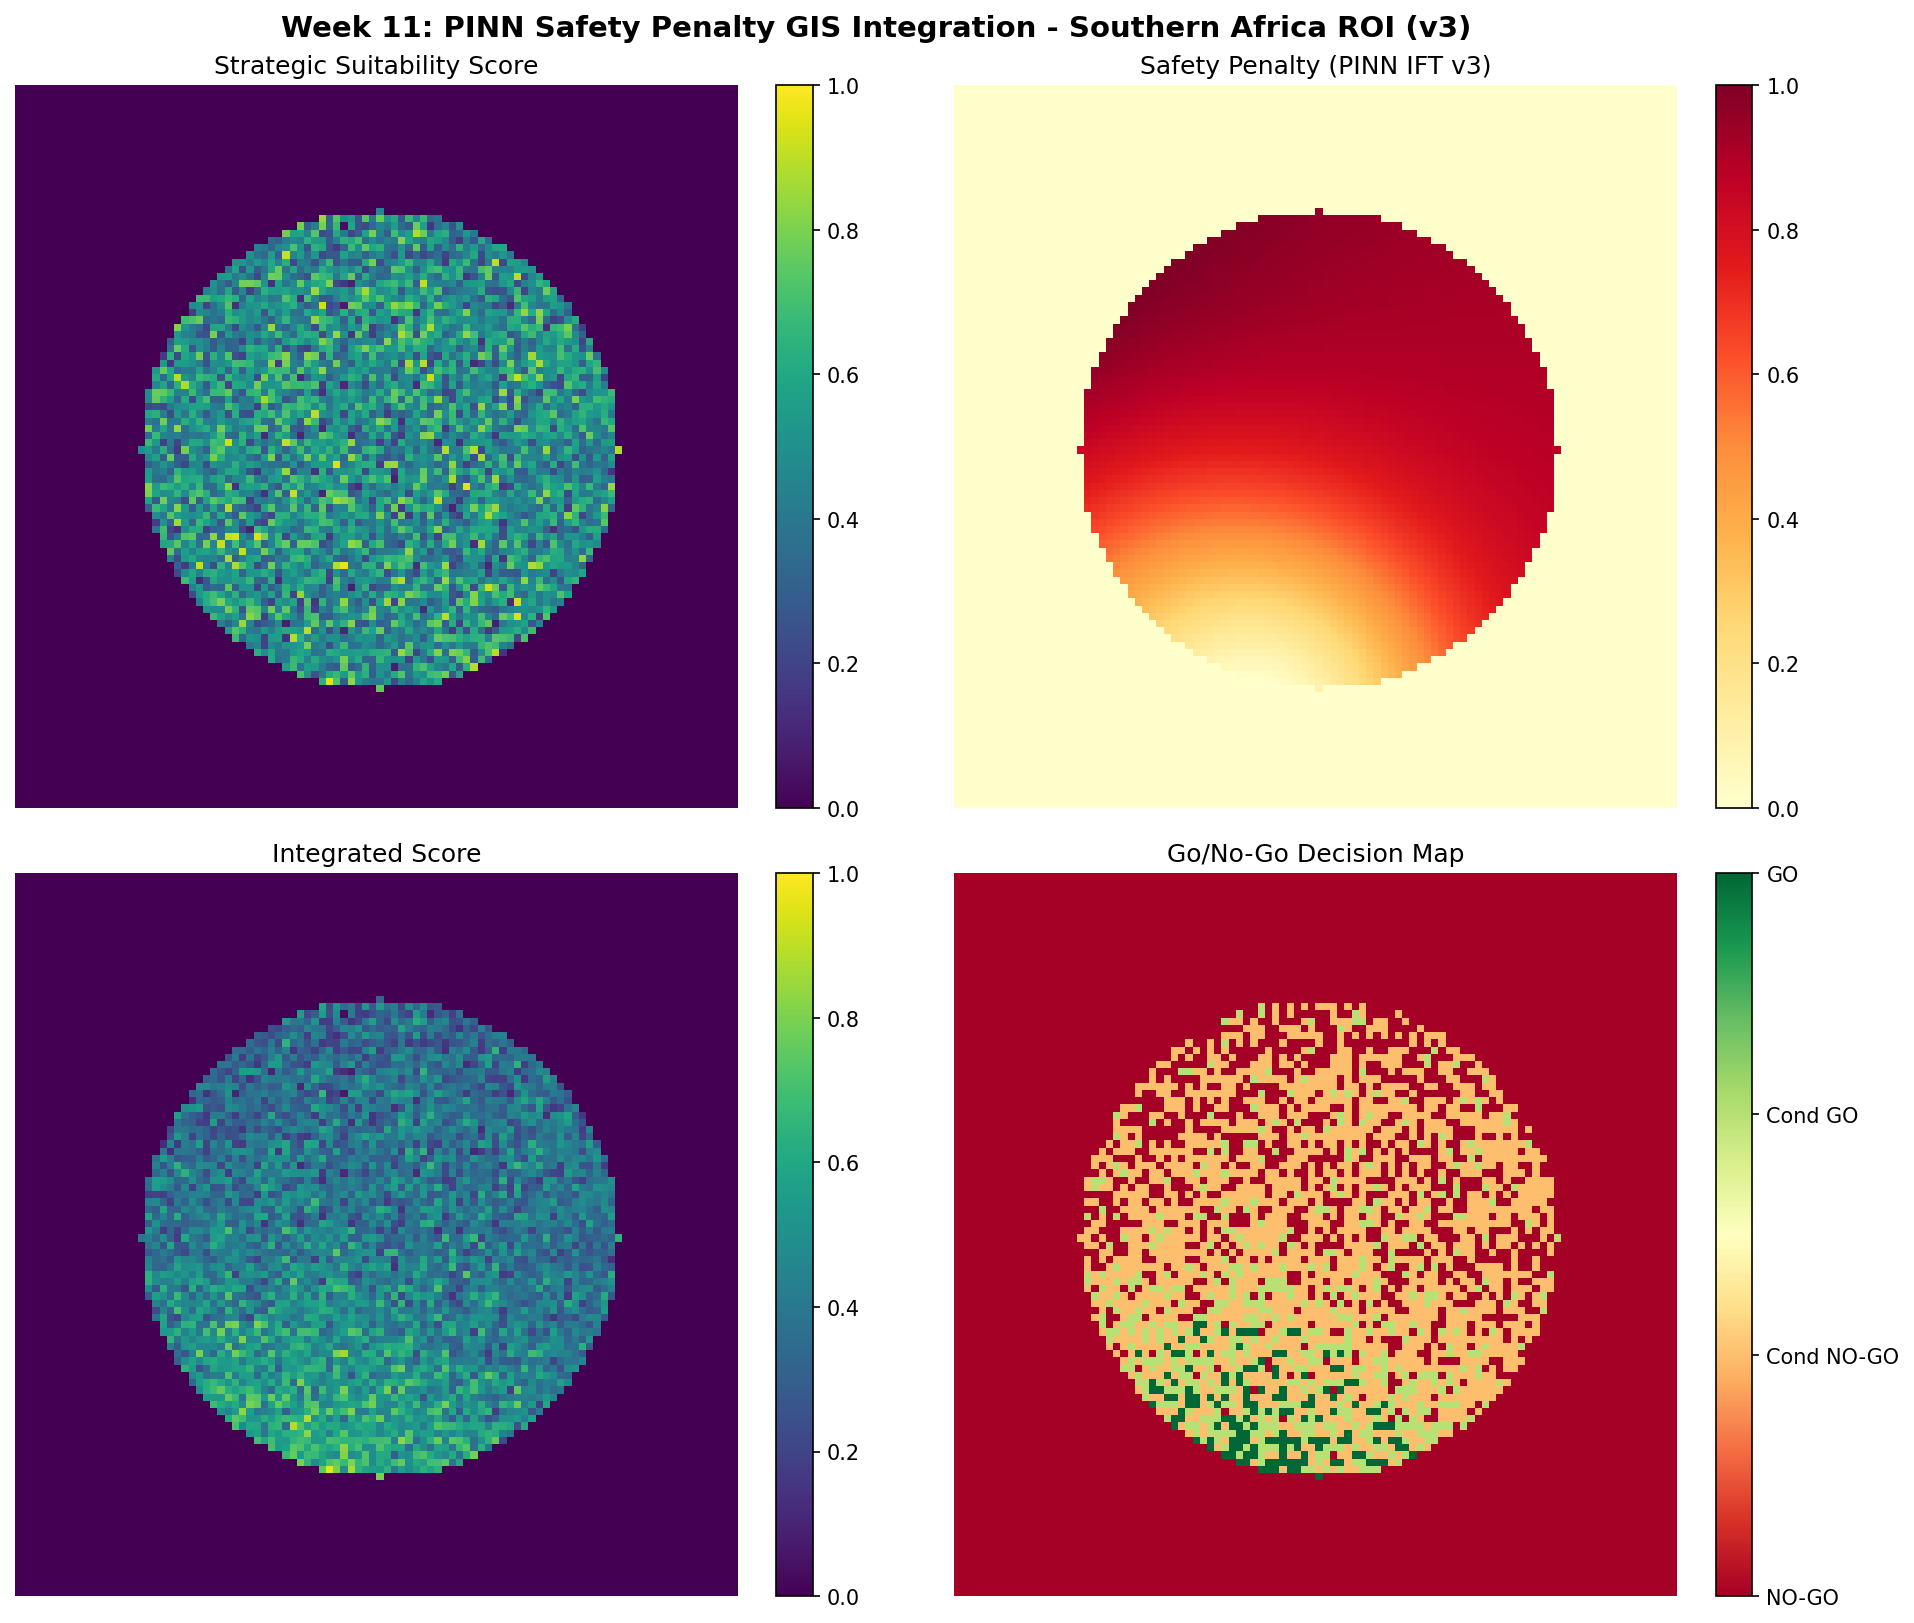
\includegraphics[width=\textwidth]{figures/week11_full_integration.png}
\caption{Week 11: PINN safety penalty GIS integration - Southern Africa ROI. Top-left: strategic suitability score; top-right: safety penalty layer; bottom-left: integrated score; bottom-right: go/no-go decision map.}
\label{fig:integration}
\end{figure}

\section{Discussion}

\subsection{Framework Evaluation}
The two-layer framework reduces investment risk by separating regional screening from site-specific physics-based safety assessment. The strategic layer rapidly narrows the search space; the tactical layer applies thermodynamic constraints where they matter most - at candidate sites. The robustness mapping (11.6\% of pixels stable across weights) provides decision-makers with confidence intervals on site selection rather than a single deterministic answer.

\subsection{Uncertainty and Limitations}
Key limitations:
\begin{itemize}
    \item \textbf{PINN training data:} The v3 model was trained on 91 experimental data points compiled from literature; while this addresses the earlier constant-output issue, the dataset remains limited in coverage of high-pressure ($>$35 MPa) and high-salinity ($>$300,000 ppm) regimes. Additional experimental validation is recommended before field deployment.
    \item \textbf{Data resolution:} The 100 $\times$ 100 grid ($\sim$0.1$^\circ$ resolution) is suitable for regional screening but requires higher-resolution data for final site selection.
    \item \textbf{Simplified reservoir conditions:} Pressure, temperature, and salinity grids were estimated from depth and geothermal gradients; site-specific measurements would improve accuracy.
\end{itemize}

\subsection{Policy and Industry Implications}
The framework supports staged investment decisions: GO zones warrant detailed site characterization; conditional GO zones require additional data before commitment; NO-GO zones can be excluded early, avoiding sunk costs. For governments in Southern Africa, the map provides a transparent, reproducible basis for hydrogen storage zoning and regulatory planning.

\section{Conclusion}

\subsection{Key Contributions}
This paper contributes:
\begin{enumerate}
    \item A two-layer decision-support framework integrating geospatial multi-objective optimization with PINN-based physics constraints for subsurface hydrogen storage site selection.
    \item A robustness mapping approach that quantifies site stability under stakeholder weight uncertainty.
    \item A PINN with Peng-Robinson EOS physics loss for H$_2$-brine IFT prediction with uncertainty quantification.
    \item Decision-ready go/no-go outputs for a Southern Africa case study, identifying two top candidate regions (Etosha and Kalahari basins).
    \item An open-source, transferable framework adaptable to other regions and storage technologies (CCS, multi-component gas).
\end{enumerate}

\subsection{Future Work}
\begin{itemize}
    \item Expansion to multi-component gas systems (H$_2$--CO$_2$--CH$_4$) and CCS applications.
    \item Integration with reservoir simulation models for injectivity and containment analysis.
    \item Real options analysis for staged investment decisions.
    \item Higher-resolution data layers for final site-scale design.
    \item Extension of experimental IFT training data to high-pressure ($>$35 MPa) and high-salinity ($>$300,000 ppm) regimes.
\end{itemize}

\section*{Acknowledgments}
The author thanks Dr. Ahmed Farid (PINNs for H$_2$-brine IFT), Pio Petro Online Internship (Hydrogen Track), University of Zimbabwe Supervisors, P. Kufamini, PhD (Research guidance), and open data providers (Global Solar Atlas, WRI Aqueduct, USGS, SEDAC).

\section*{Code and Data Availability}
Framework code, trained models, and data are available at:
\url{https://github.com/kudakwashedouglas/hydrogen_storage_site_selection}

\section*{References}
\begin{thebibliography}{9}

\bibitem{ai2026}
Ai, L., \& Trusler, J.~P.~M. (2026).
Experimental study of hydrogen-brine interfacial tension: Implications for natural hydrogen production.
\textit{International Journal of Hydrogen Energy}. \url{https://doi.org/10.1016/j.ijhydene.2026.154442}

\bibitem{farid2026}
Farid, A. (2026).
Physics-informed model for H$_2$-brine interfacial tension prediction outside the development range: Hydrogen storage implications.
\textit{Results in Engineering}.

\bibitem{hosseini2022}
Hosseini, M. (2022).
Experimental investigation of the interface and wetting characteristics of rock-H$_2$-brine systems for H$_2$ geological storage.
Edith Cowan University thesis.

\bibitem{omrani2023}
Omrani, S., Ghasemi, M., Singh, M., Mahmoodpour, S., \& Zhou, T. (2023).
Interfacial Tension--Temperature--Pressure--Salinity Relationship for the Hydrogen--Brine System under Reservoir Conditions: Integration of Molecular Dynamics and Machine Learning.
\textit{Langmuir}, 39(36), 12680--12694.

\bibitem{solar}
Global Solar Atlas. \url{https://globalsolaratlas.info}

\bibitem{wri}
WRI Aqueduct Water Risk Atlas. \url{https://www.wri.org/aqueduct}

\bibitem{usgs}
USGS World Petroleum Assessment. \url{https://pubs.usgs.gov}

\bibitem{sedac}
SEDAC Population Density. \url{https://sedac.ciesin.columbia.edu}

\end{thebibliography}

\end{document}